\documentclass[a4paper,12pt]{article}

\usepackage[top = 2cm, bottom = 2cm, left = 2cm, right = 2cm]{geometry} 

\usepackage[T1]{fontenc}
\usepackage[utf8]{inputenc}
\usepackage[spanish]{babel}
\usepackage{multirow}
\usepackage{booktabs} 
\usepackage{graphicx} 
\usepackage{setspace}
\setlength{\parindent}{0in}
\usepackage{float}
\usepackage{fancyhdr}
\usepackage{enumitem}
\usepackage{tikz-timing}
\usepackage{amsmath,amssymb,amsfonts}
\usepackage{hyperref} % Support for hyperlinks
\usepackage{wrapfig}
\usepackage{xcolor}

\tikzset{
timing/z/.style={color=red},
timing/l/.style={color=red},
timing/h/.style={color=red},
timing/slope=0,
timing/name/.append style={yshift=1.5mm}
}

\pagestyle{fancy} 
\fancyhf{} .
\lhead{\footnotesize Introducción al Software de Entretenimiento: Laboratorio 2}

\rhead{\footnotesize 20 de septiembre del 2020}

\cfoot{\footnotesize \thepage} 

\begin{document}

\thispagestyle{empty}

\begin{tabular}{p{15.5cm}} 
\large Universidad Nacional de San Agustín \\ 
\large Facultad de Ingeniería de Producción y Servicios \\
\large Escuela Profesional de Ingeniería de Sistemas \\
{\LARGE \bf Introducción al Software de Entretenimiento} \\
\vspace{1mm}
Alumno: Mestas Escarcena, Carlos Alberto \\
Grupo: A \\
\hline \\
\end{tabular} 

\begin{center} 
	{\LARGE \bf Laboratorio 2}
	\vspace{2mm}
\end{center}  

El desarrollo de este informe se puede encontrar en el repositorio de \textcolor{blue}{
    \href{https://github.com/CarlosMestas/IDSE_CarlosMestas_Laboratorio2}{GitHub}} y los videos con una mayor explicación en \textcolor{blue}{
    \href{https://drive.google.com/drive/folders/1o1PGTRtjRTngNK9nAKqZac3Yk3iThDme?usp=sharing}{Google Drive}}, el primer video grabado trata acerca del desarrollo del nivel y el segundo video con una demostración de como superar el nivel.
    
\section*{Desarrollo}

    \begin{figure}[ht]
        \centering                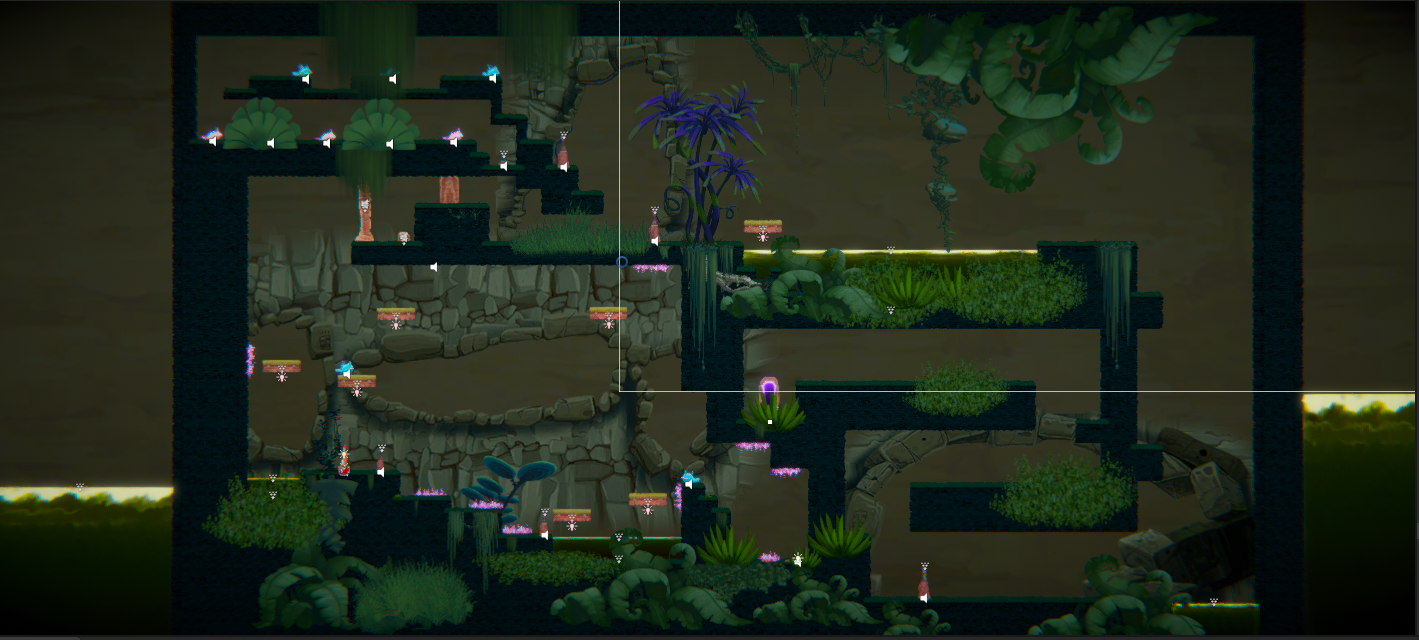
\includegraphics[width=1\textwidth]{images/CaptureIDSE01.PNG}
        \caption{Visualización completa del nivel.}
    \end{figure}

    Para el desarrollo del nivel en general se a trabajo ordenando capas, por ejemplo nuestro personaje tiene un valor de 4, el veneno cuenta con el mismo valor, la vegetación tiene un valor un poco más alto y de la misma forma en todo el nivel.
    \\
    \\
    Se le agregó también en el nivel el sonido por defecto que se encuentra en el paquete de desarrollo, así como también se modificó la coloración de todos los objetos en general, el suelo, el fondo, las cavernas que se pueden visualizar y también la coloración de las plantas.
    \\
    \\
    Se observa también en esta imagen que se tienen una serie de plataformas, estan van a servir para poder pasar la primera parte de este nivel, se tiene que tener cuidado con ellas ya que se encuentran distintas partes y también un enemigo.
\clearpage
\newpage

    \begin{figure}[ht]
        \centering                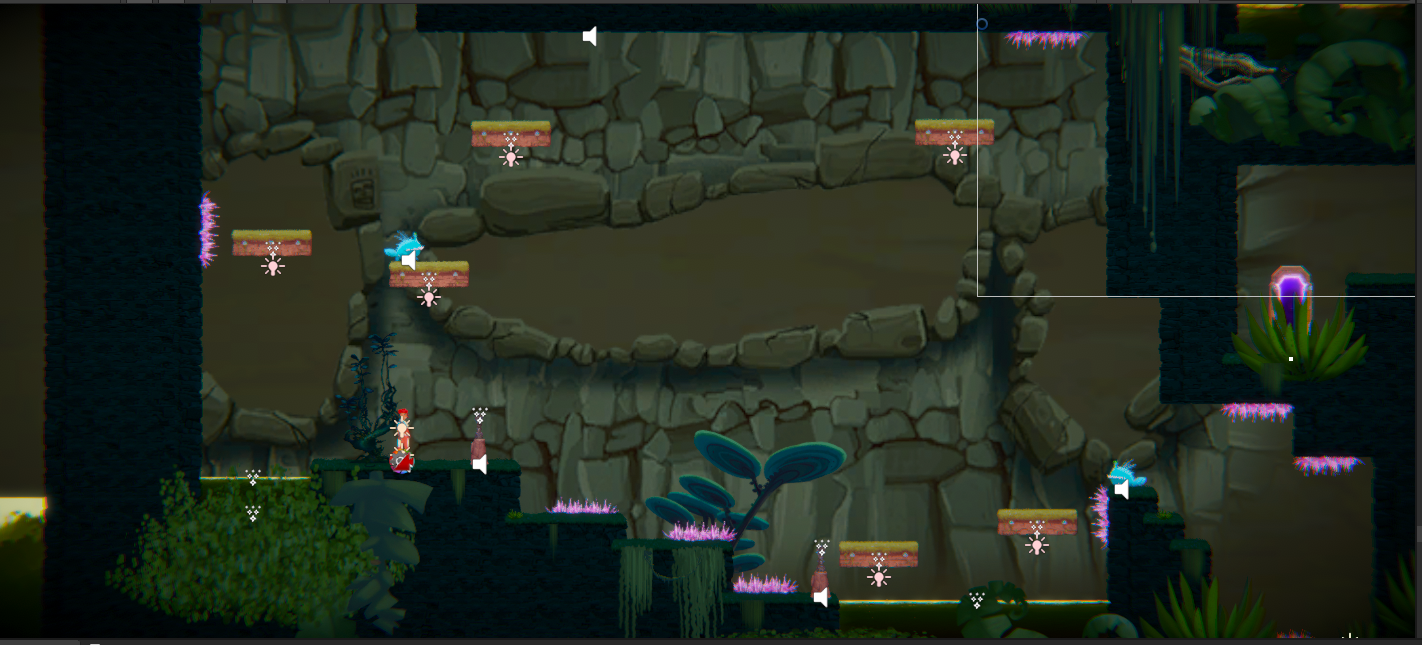
\includegraphics[width=1\textwidth]{images/CaptureIDSE02.PNG}
        \caption{Primera parte del nivel.}
    \end{figure}    
    
    En la primera parte comenzamos con un poste de información que nos va a dar la bienvenida al juego y que el objetivo principal de este nivel es poder llevar a Ellen al transportador, este poste de información como el resto se complementa con un \textit{DialogCanvas} que nos permite realizar esta interacción para el cuadro de diálogo, estos postes están programados para mostrar el mensaje al momento de que nos acercamos y al momento de alejarnos desaparecen luego de dos segundos, tenemos luego los primeros obstáculos que tendremos que superar son espinas, teniendo cuidado entonces en nuestro salto, luego podemos observar un segundo poste de información que nos da una indicación de con que teclas vamos a poder usar las armas, ya que podemos ver del otro lado nuestro primer enemigo, el primer enemigo que tenemos es un \textit{Spitter} estos enemigos están programados con dos puntos de vida y un rango de visión solo para objetivos que estén delante suyo, tenemos que tener cuidado con las espinas ya que la plataforma nos lleva hacia ellas y podemos perder un punto de vida.

    \begin{figure}[ht]
        \centering                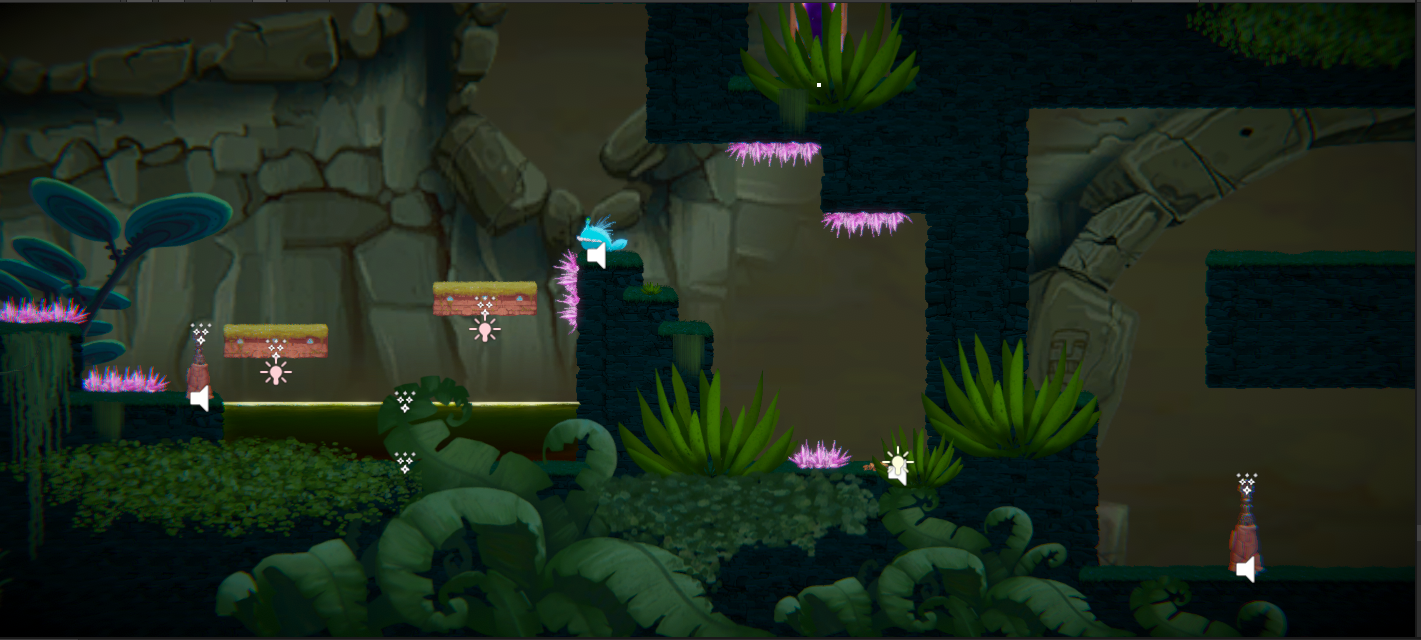
\includegraphics[width=1\textwidth]{images/CaptureIDSE03.PNG}
        \caption{Visualización de la caverna tras el enemigo.}
    \end{figure}  

    Detrás del \textit{Spitter} podemos observar escondido entre las plantas un botón en el suelo que nos sirve para poder mover una puerta que se encuentra en la parte de arriba, en el caso de que el jugador decida no pasar por esta zona entonces tendrá que regresar al inicio y pisar este botón.

    \begin{figure}[ht]
        \centering                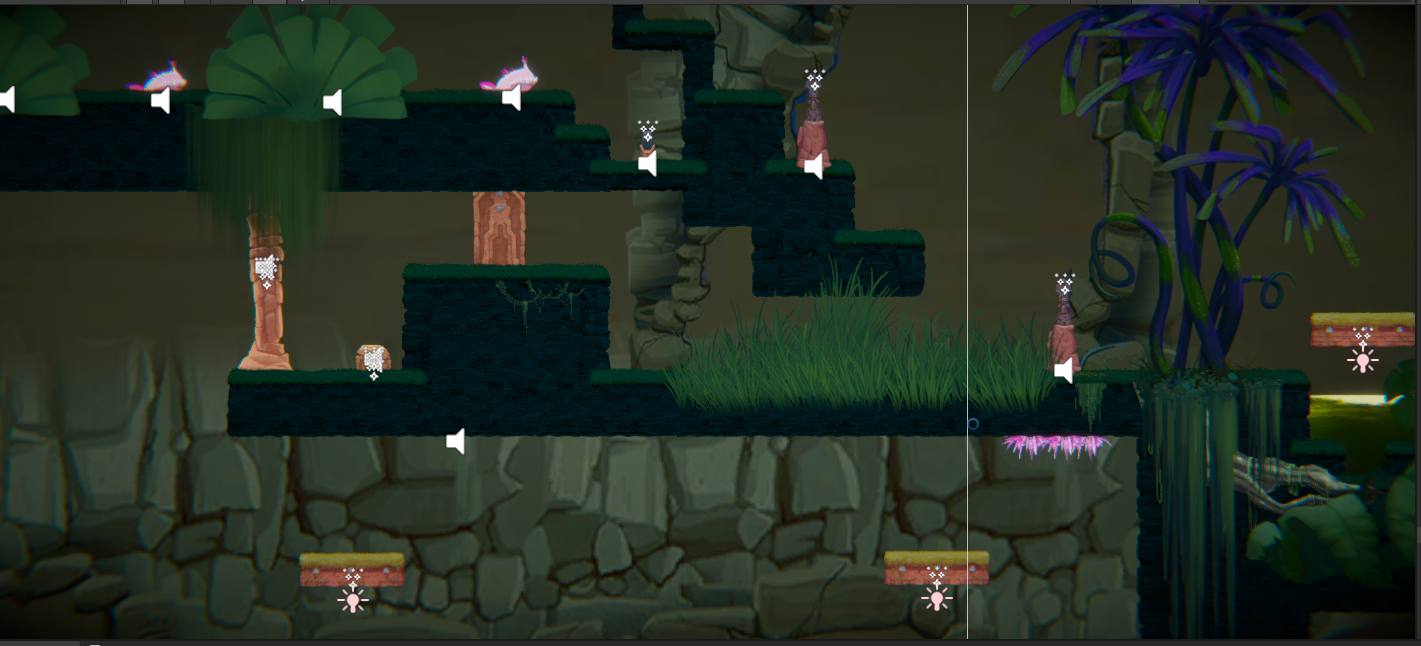
\includegraphics[width=1\textwidth]{images/CaptureIDSE04.PNG}
        \caption{Obstáculo para destruir y la puerta.}
    \end{figure}  
    
    Tenemos en esta parte una columna para destruir, esta destrucción se puede realizar mediante un salto y golpe de sable, luego de esta columna observamos un pequeña caja donde podemos encontrar un punto de vida de salud que se activará automáticamente al pasar por ahí en caso de que hayamos perdido salud en la parte inferior, aquí también podemos observar un poste de información que nos indicará que tenemos que buscar la forma de activar la plataforma para esquivar el ácido.

    \begin{figure}[ht]
        \centering                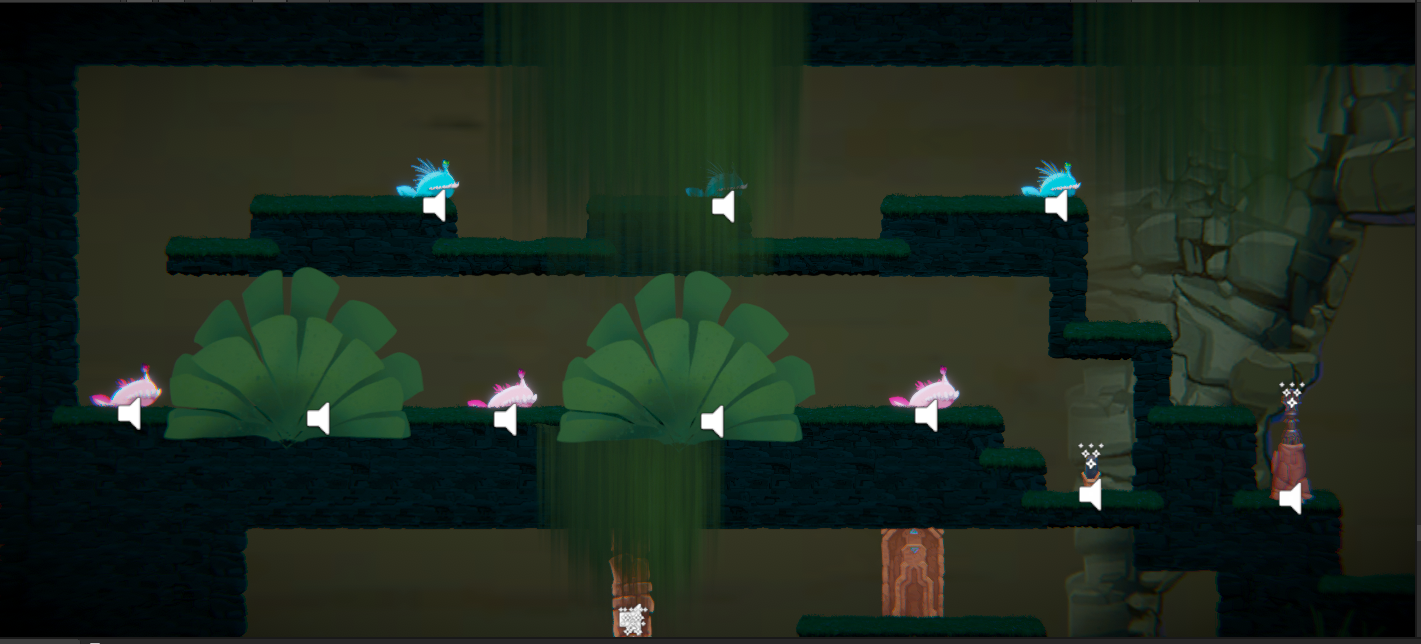
\includegraphics[width=1\textwidth]{images/CaptureIDSE05.PNG}
        \caption{Conjunto de enemigos.}
    \end{figure}     
    
    Para poder activar la plataforma antes mencionada usaremos un \textit{SingleUseSwitch} que esta custodiada por enemigos, el poste de información de acá nos indica que tenemos que tener cuidado con los enemigos que se pueden ocultar, esto se debe a la vegetación que oculta a los enemigos, acá también vemos un nuevo enemigo, un \textit{Chomper} que a diferencia del otro este no ataca de lejos, pero si tiene en este caso un radio de visión de 360º.
    
\clearpage
\newpage

    \begin{figure}[ht]
        \centering                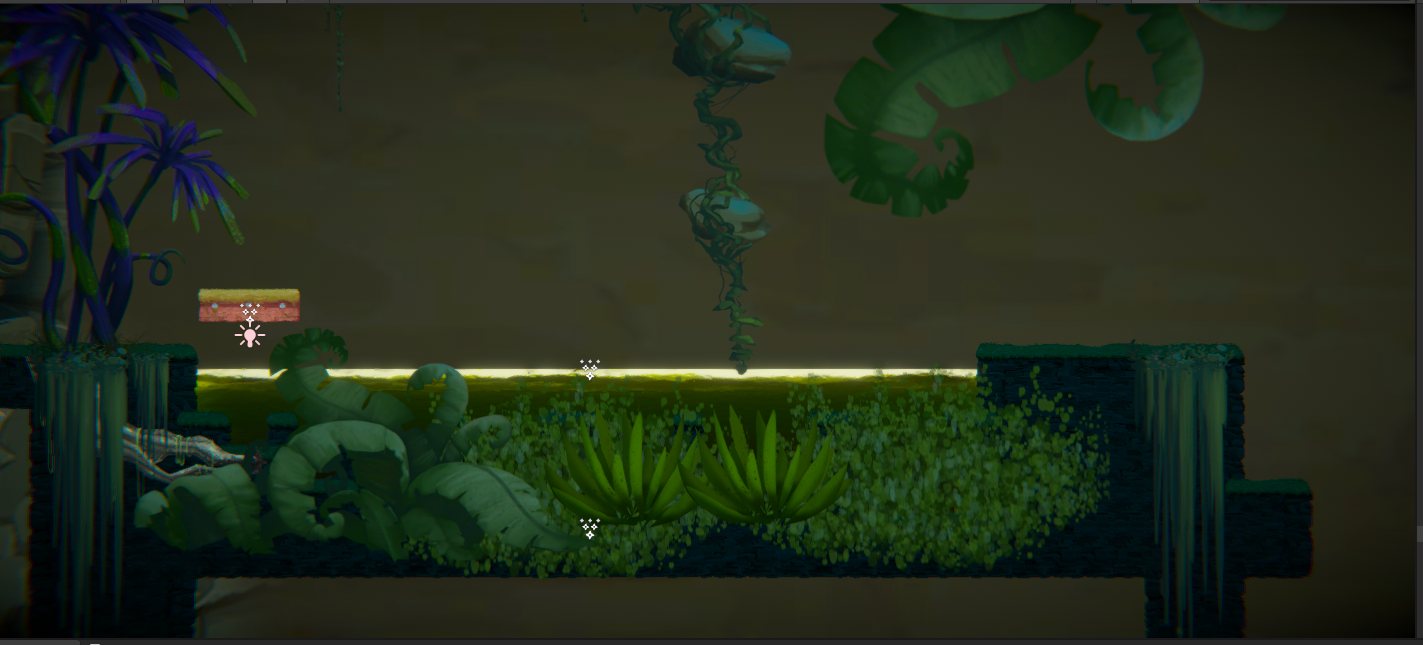
\includegraphics[width=1\textwidth]{images/CaptureIDSE06.PNG}
        \caption{Plataforma con activación.}
    \end{figure}     
    
    Al activar esta plataforma previamente ya podemos superar esta parte del nivel.
    
    \begin{figure}[ht]
        \centering                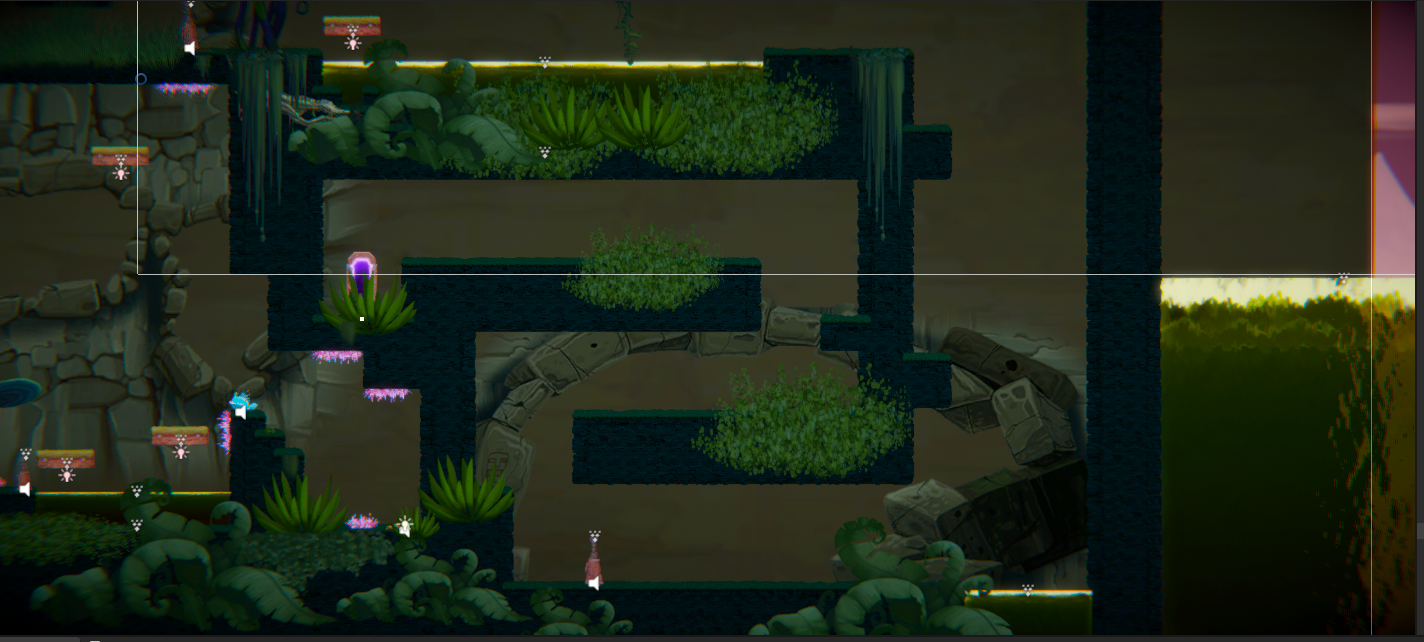
\includegraphics[width=1\textwidth]{images/CaptureIDSE07.PNG}
        \caption{Parte final.}
    \end{figure}     
    
    Finalmente tenemos que descender con un poco de cuidado con el ácido y luego nos vamos para la izquierda donde tendremos el último poste de información que nos indica que tenemos que tener cuidado con los enemigos ocultos, que pasemos solamente cuando estemos seguros de que ya no hay ninguno, esto se debe a que aquí en encontramos dos \textit{EnemySpawener} ocultos entre la vegetación, donde aparecerá un enemigo cada que otro muera, con un máximo de 5 y con un tiempo de aparición de 1 segundo. Luego de superar estos obstáculos termina el nivel con un \textit{teleporter}, este se tendrá que activar con la letra \textit{e}, esta indicación también aparecerá en un cuadro de diálogo, este \textit{teleporter} nos llevará al nivel final del juego que estaba previamente desarrollado.

\end{document}
